%\title{LaTeX Portrait Poster Template}
%%%%%%%%%%%%%%%%%%%%%%%%%%%%%%%%%%%%%%%%%

%----------------------------------------------------------------------------------------
%	PACKAGES AND OTHER DOCUMENT CONFIGURATIONS
%----------------------------------------------------------------------------------------

\documentclass[a0,portrait]{a0poster}

\usepackage{multicol} % This is so we can have multiple columns of text side-by-side
\columnsep=100pt % This is the amount of white space between the columns in the poster
\columnseprule=3pt % This is the thickness of the black line between the columns in the poster

\usepackage[svgnames]{xcolor} % Specify colors by their 'svgnames', for a full list of all colors available see here: http://www.latextemplates.com/svgnames-colors

\usepackage{times} % Use the times font

\usepackage{graphicx} % Required for including images
\graphicspath{{figures/}} % Location of the graphics files

\usepackage{booktabs} % Top and bottom rules for table
\usepackage[font=small,labelfont=bf]{caption} % Required for specifying captions to tables and figures
\usepackage{amsfonts, amsmath, amsthm, amssymb} % For math fonts, symbols and environments
\usepackage{wrapfig} % Allows wrapping text around tables and figures

% Include any extra LaTeX packages required
\usepackage[square, numbers, comma, sort&compress]{natbib}  % Use the "Natbib" style for the references in the Bibliography

\usepackage{natbib}
\usepackage{url}
%\hypersetup{urlcolor=blue, colorlinks=true}  


\usepackage [english]{babel}
\usepackage [autostyle, english = american]{csquotes}
\MakeOuterQuote{"}

\begin{document}

%----------------------------------------------------------------------------------------
%	POSTER HEADER 
%----------------------------------------------------------------------------------------

% The header is divided into two boxes:
% The first is 75% wide and houses the title, subtitle, names, university/organization and contact information
% The second is 25% wide and houses a logo for your university/organization or a photo of you
% The widths of these boxes can be easily edited to accommodate your content as you see fit

\begin{minipage}[b]{0.75\linewidth}
\VeryHuge \color{NavyBlue} \textbf{Clustering, Teleconnectivity and \\Webdevelopment} \color{Black}\\ % Title
\Huge\textit{latest work}\\[2.4cm] % Subtitle
\huge \textbf{Benjamin T. Schwertfeger}\\[0.5cm] % Author(s)
\huge Alfred-Wegener-Institute Bremerhaven\\[0.4cm] % 
\Large \texttt{benjamin.schwertfeger@awi.de}
\end{minipage}
%
\begin{minipage}[b]{0.25\linewidth}

\includegraphics[width=14cm]{awilogo.png}\ 
\end{minipage}

\vspace{1cm} % A bit of extra whitespace between the header and poster content

%----------------------------------------------------------------------------------------

\begin{multicols}{3} % This is how many columns your poster will be broken into, a portrait poster is generally split into 2 columns

%----------------------------------------------------------------------------------------
%	ABSTRACT
%----------------------------------------------------------------------------------------

\color{Navy} % Navy color for the abstract

\begin{abstract}
This poster shows the actual status, as well as parts of the results of my work, which I have achieved during the last year here at AWI. This includes statistical analyses, as well as methods for creating and evaluating clusters, and teleconnections based on correlation. I have also recently been working on the creation of websites in a scientific context. My supervisor is Gerrit Lohmann.
\end{abstract}
%----------------------------------------------------------------------------------------
%	About me
%----------------------------------------------------------------------------------------
\color{Black} % SaddleBrown color for the introduction
%\begin{center}
\section*{\centering About me}
%\end{center}
I study business informatics at the University of Bremerhaven and worked as an intern and now again as a \grqq{}HiWi\grqq{} at the Alfred-Wegener-Institute Bremerhaven in the area of climate science - section \grqq{}Paleo-climate Dynamics\grqq{}.
I really like programming, especially in Python, JavaScript and C++ and look forward to every new project.\\

%----------------------------------------------------------------------------------------
%	Analysis and comparison of multiple climate models
%----------------------------------------------------------------------------------------

\color{Black} % SaddleBrown color for the introduction
\section{Analysis and comparison of multiple climate models}
Besides the statistical analysis of global (CMIP6-MPI-M-ESM-LR), regional (CORDEX-MPI-M-ESM-1-2-LR), bais corrected and observed data for the region Europe, I have used further methods like cluster analysis and created a method for the detection and visualization of teleconnections. Later I also worked with data from the LGM MIS33 and PI runs in the global scale. 

%----------------------------------------------------------------------------------------
%	ANOMALIES AND SIGNIFICANCE
%----------------------------------------------------------------------------------------

\color{Black} % DarkSlateGray color for the rest of the content
\subsection{Anomalies and significance}
At the beginning of my work at AWI, I was quite inexperienced and so I compared and plotted a lot of data and looked for differences and special features. This helped me a lot to learn how to use certain tools and methods.
\begin{center}\vspace{1cm}
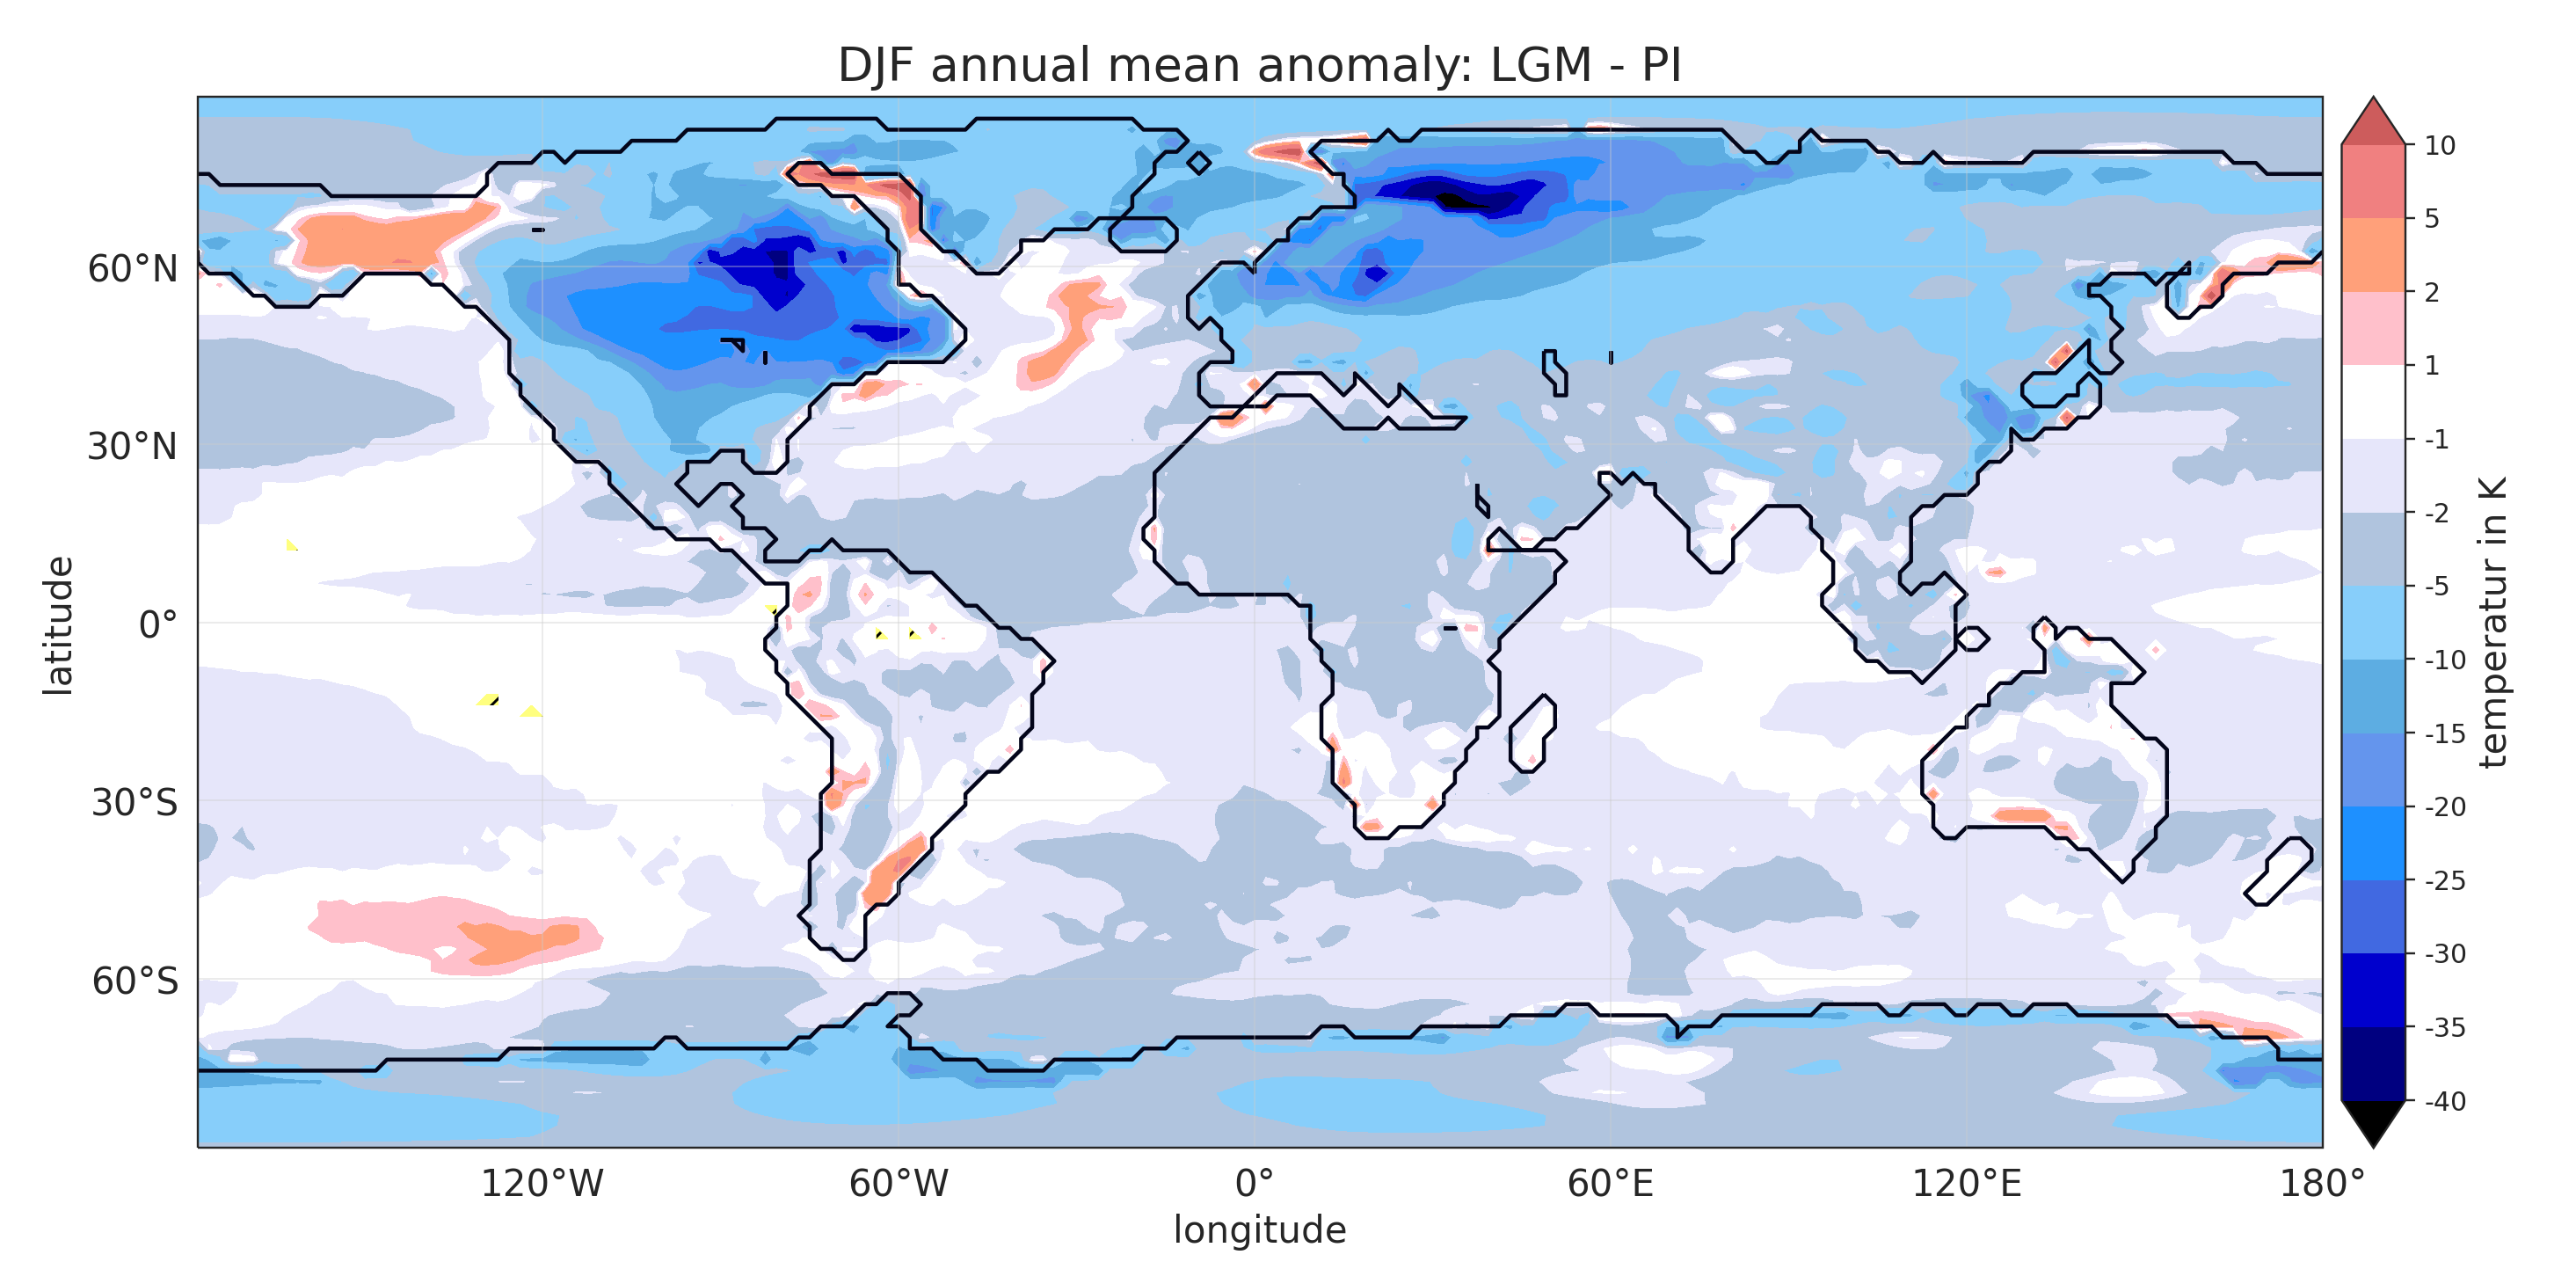
\includegraphics[width=1\linewidth]{lgmpisig.png}
\label{fig:lgmpisig}
\captionof{figure}{\color{Green} Difference in annual mean surface temperatures between the LGM and PI run (90 years); yellow shaded areas are are non-significant}
\end{center}\vspace{1cm}

Such and other plots are also available for the Africa and Europe regions on various models.\\
In my analysis of the european data, the focus was on the efficiency of the bias correction. There, it was shown that corrected data resemble the observed data significantly more than uncorrected data.

%----------------------------------------------------------------------------------------
%	CLUSTERING
%----------------------------------------------------------------------------------------

\color{Black} % DarkSlateGray color for the rest of the content

\subsection{Clustering}
In the correlation-based clustering procedure, similarly correlated locations are assigned to the same clusters. This is based on annual mean temperatures over a period of at least 30 years. One of the objectives of the cluster analyses is to determine the degrees of freedom.

\begin{center}\vspace{1cm}
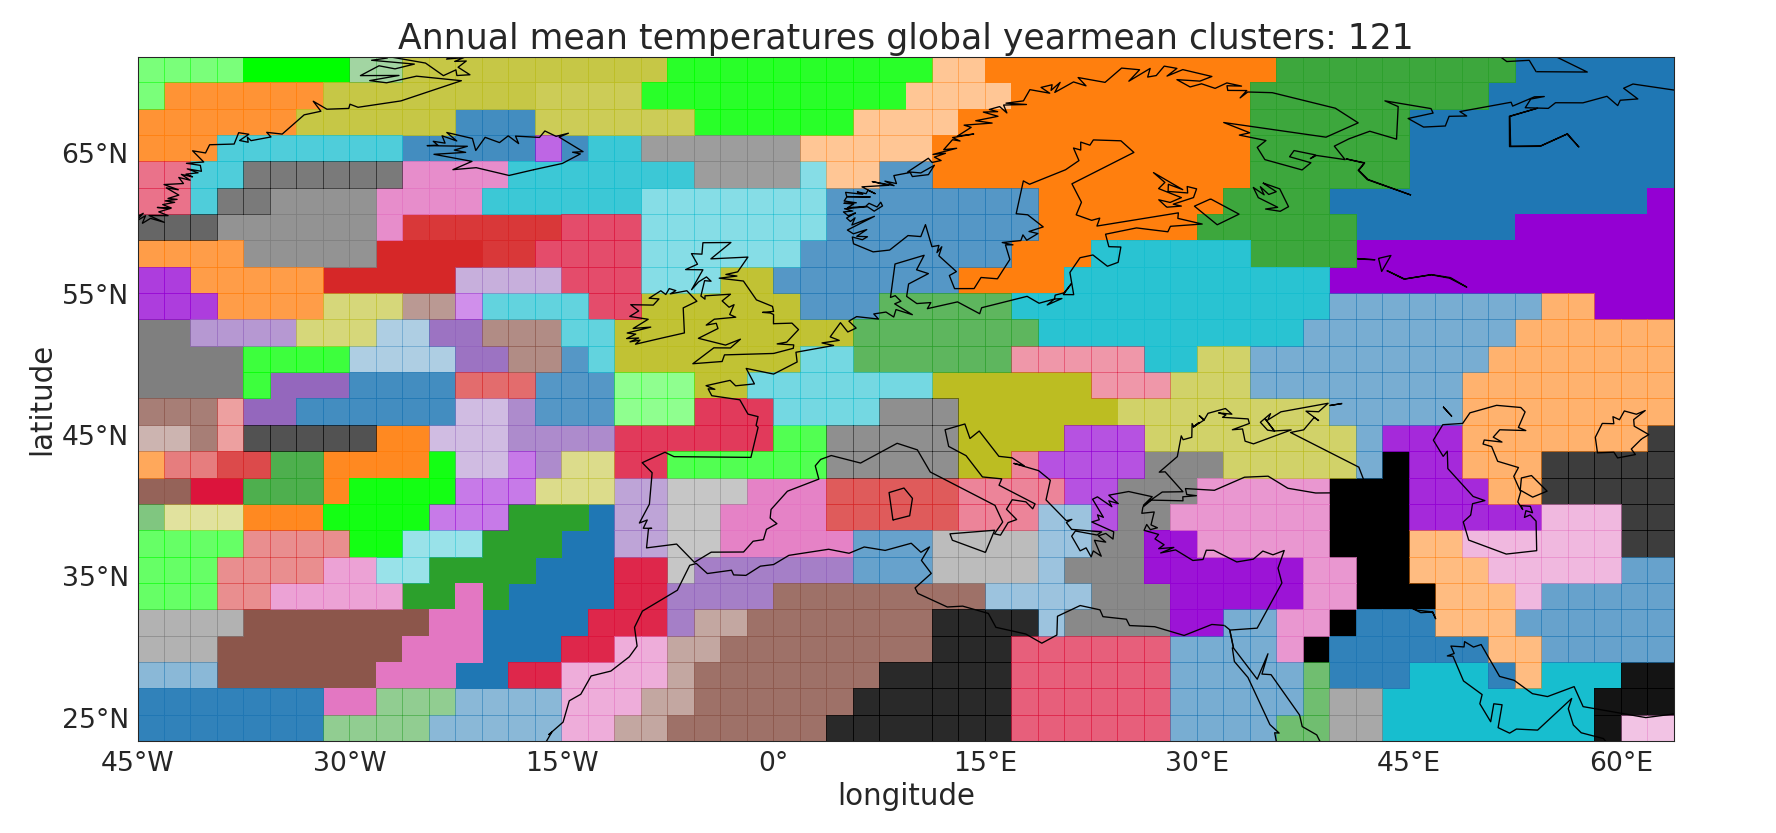
\includegraphics[width=1\linewidth]{globtascluster.png}
\captionof{figure}{\color{Green} Clusters of annual mean temperatures between 1971-2000 in Europe in CMIP6 MPI-ESM-1-2-LR\_r1i1p1f1.}
\end{center}\vspace{1cm}

During the examination of the european area, it was visually noticeable that more clusters are found on the water than on the land. This was confirmed after a further examination. 

%----------------------------------------------------------------------------------------
% TELECONNECTIVITY
%----------------------------------------------------------------------------------------

\subsection{Teleconnectivity}
I have developed a method to detect teleconnections - similar to the one described in \cite{teleconn}. This involves connections between locations that have strong negative correlations to each other.

\begin{center}\vspace{1cm}
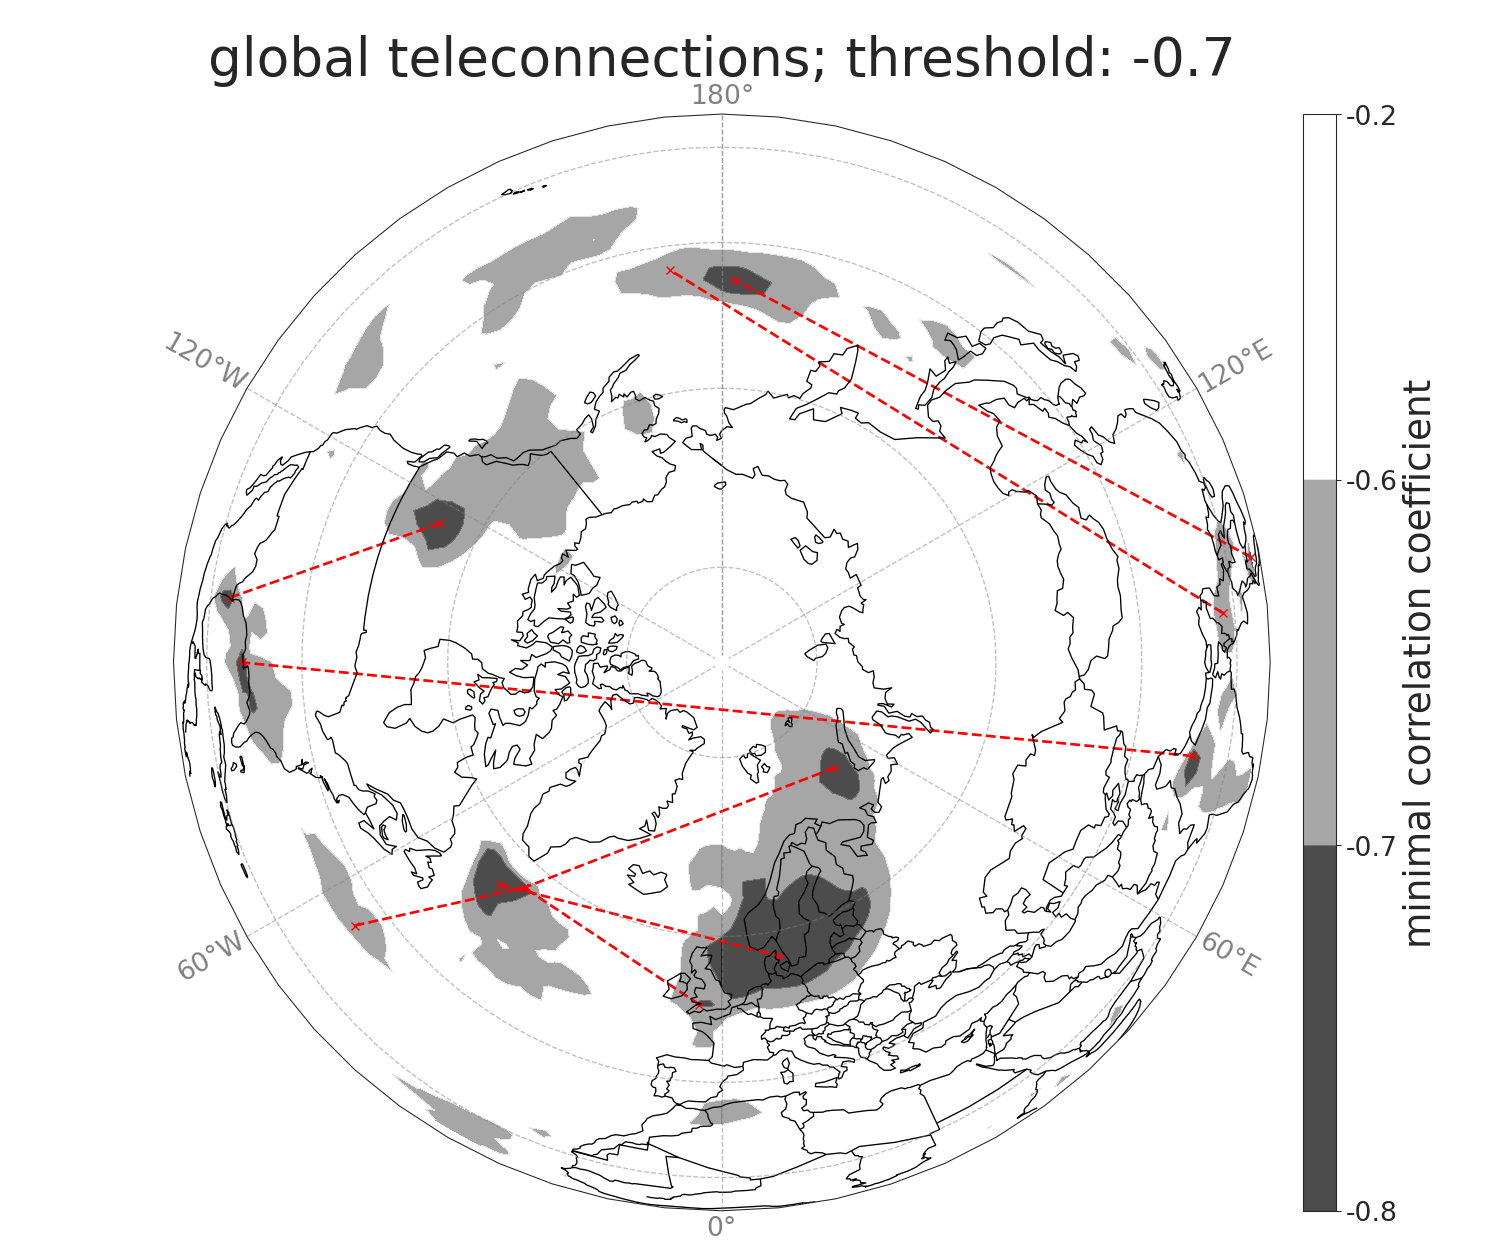
\includegraphics[width=1.0\linewidth]{globalteleconn.png}
\captionof{figure}{\color{Green}The contour plot represents the minimum one-point correlation for all locations, which are divided into three contour levels. Red dotted lines show the teleconnections between centers of strongly negatively correlated areas. (northern hemisphere of annual mean temperatures for years 1971-2000 in CMIP6 MPI-ESM-1-2-LR-r1i1p1f1)}
\end{center}\vspace{1cm}

During the analysis of the teleconnections, for example, it was noticed that the bias correction had too strong an influence on the amplitude of the temperatures, so that no representative teleconnections could be found.

Despite the (so far) erroneous data from LGM, MIS3 and PI, it was shown that there were many more and stronger teleconnections in the LGM run, whereas the PI run had much higher correlation values.

%------------------------------------------------

\section{Web Development}
Since I work in the field of IT and like to look around in all directions and started to create websites with scientific graphics to allow easy access and retrieval of data.

\subsection{Energy Balance Models}
Gerrit asked me to create something illustrative about energy balance models, because he wanted to give his students something interactive to take away with them. So I built a website on which you can run and visualize a simple and a more complex energy balance model with different parameters.

\begin{center}\vspace{1cm}
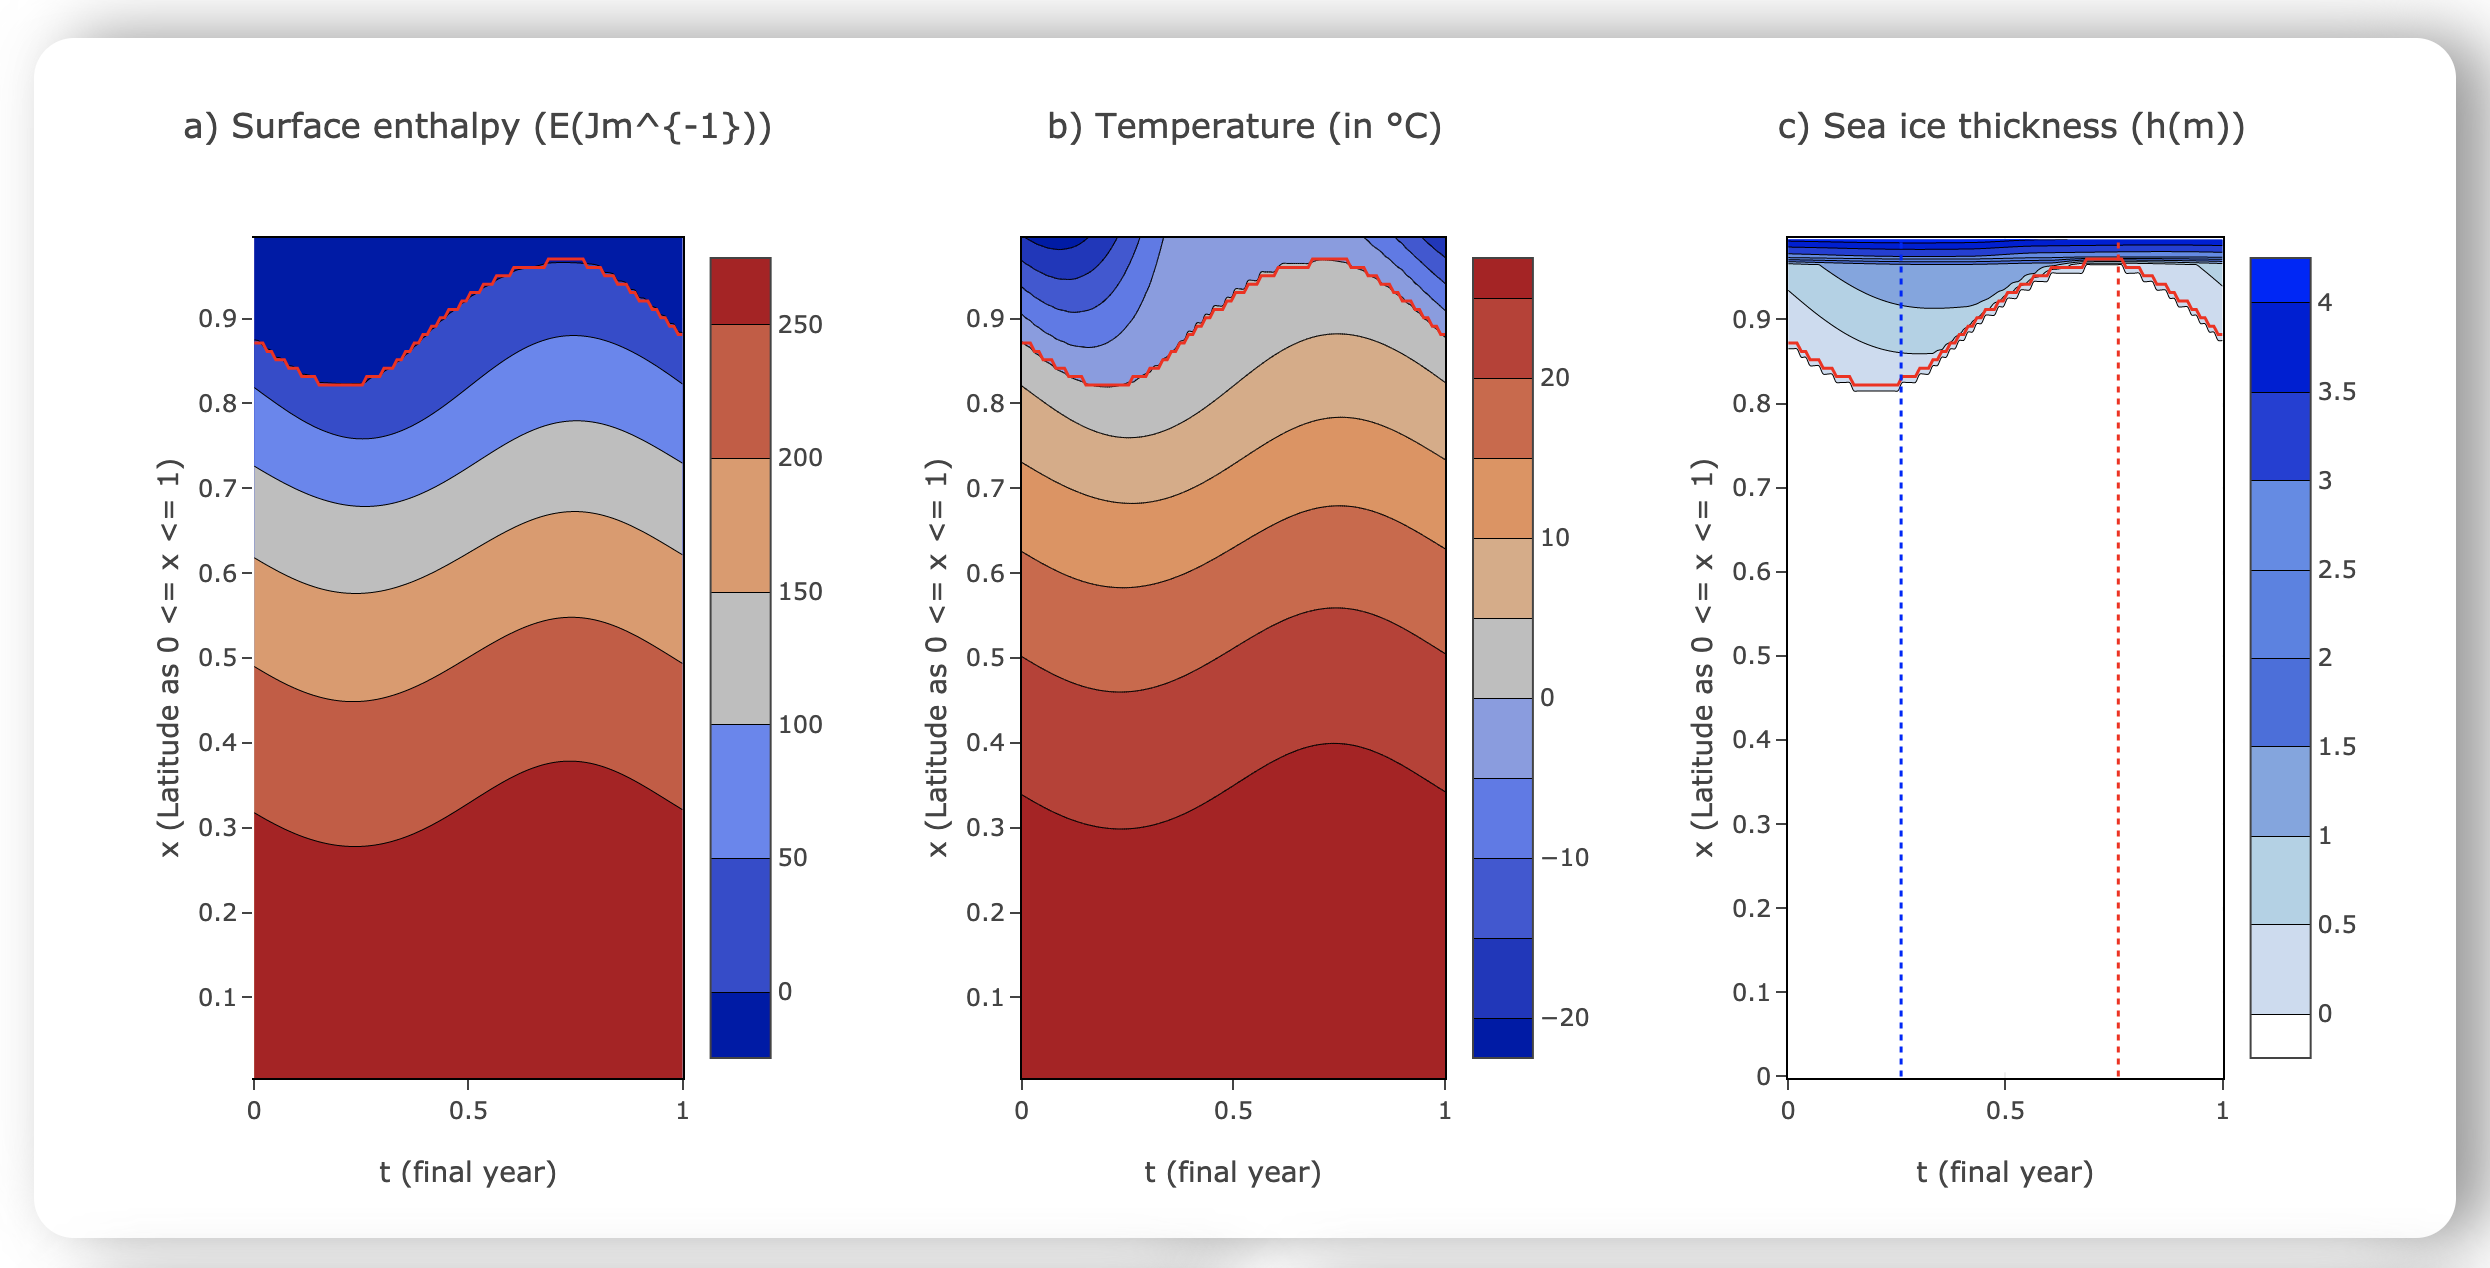
\includegraphics[width=0.8\linewidth]{complexebm.png}
\captionof{figure}{\color{Green} Section of the results of a complex EBM run; seasonal cycle of (a) surface enthalpy \(E(Jm^{-2})\), (b) temperatures, (c) sea ice edge and thickness; red line = ice edge; red dashed line: midsummer; blue dashed line: midwinter}
\end{center}\vspace{1cm}

The models implemented there are variations of the ones described in \cite{ebmsite}.

\subsection{Daisyworld}
After the website with the energy balance models was so well received, I came across the Daisyworld model described in \cite{daisyworld}, which Gerrit has also included in his lectures. 

Daisyworld is a theoretical cloudless planet with negligible greenhouse gases where only black and white daisies live. The white ones have a higher albedo than the black ones. Together they regulate the energy balance on the planet.
\begin{center}\vspace{1cm}
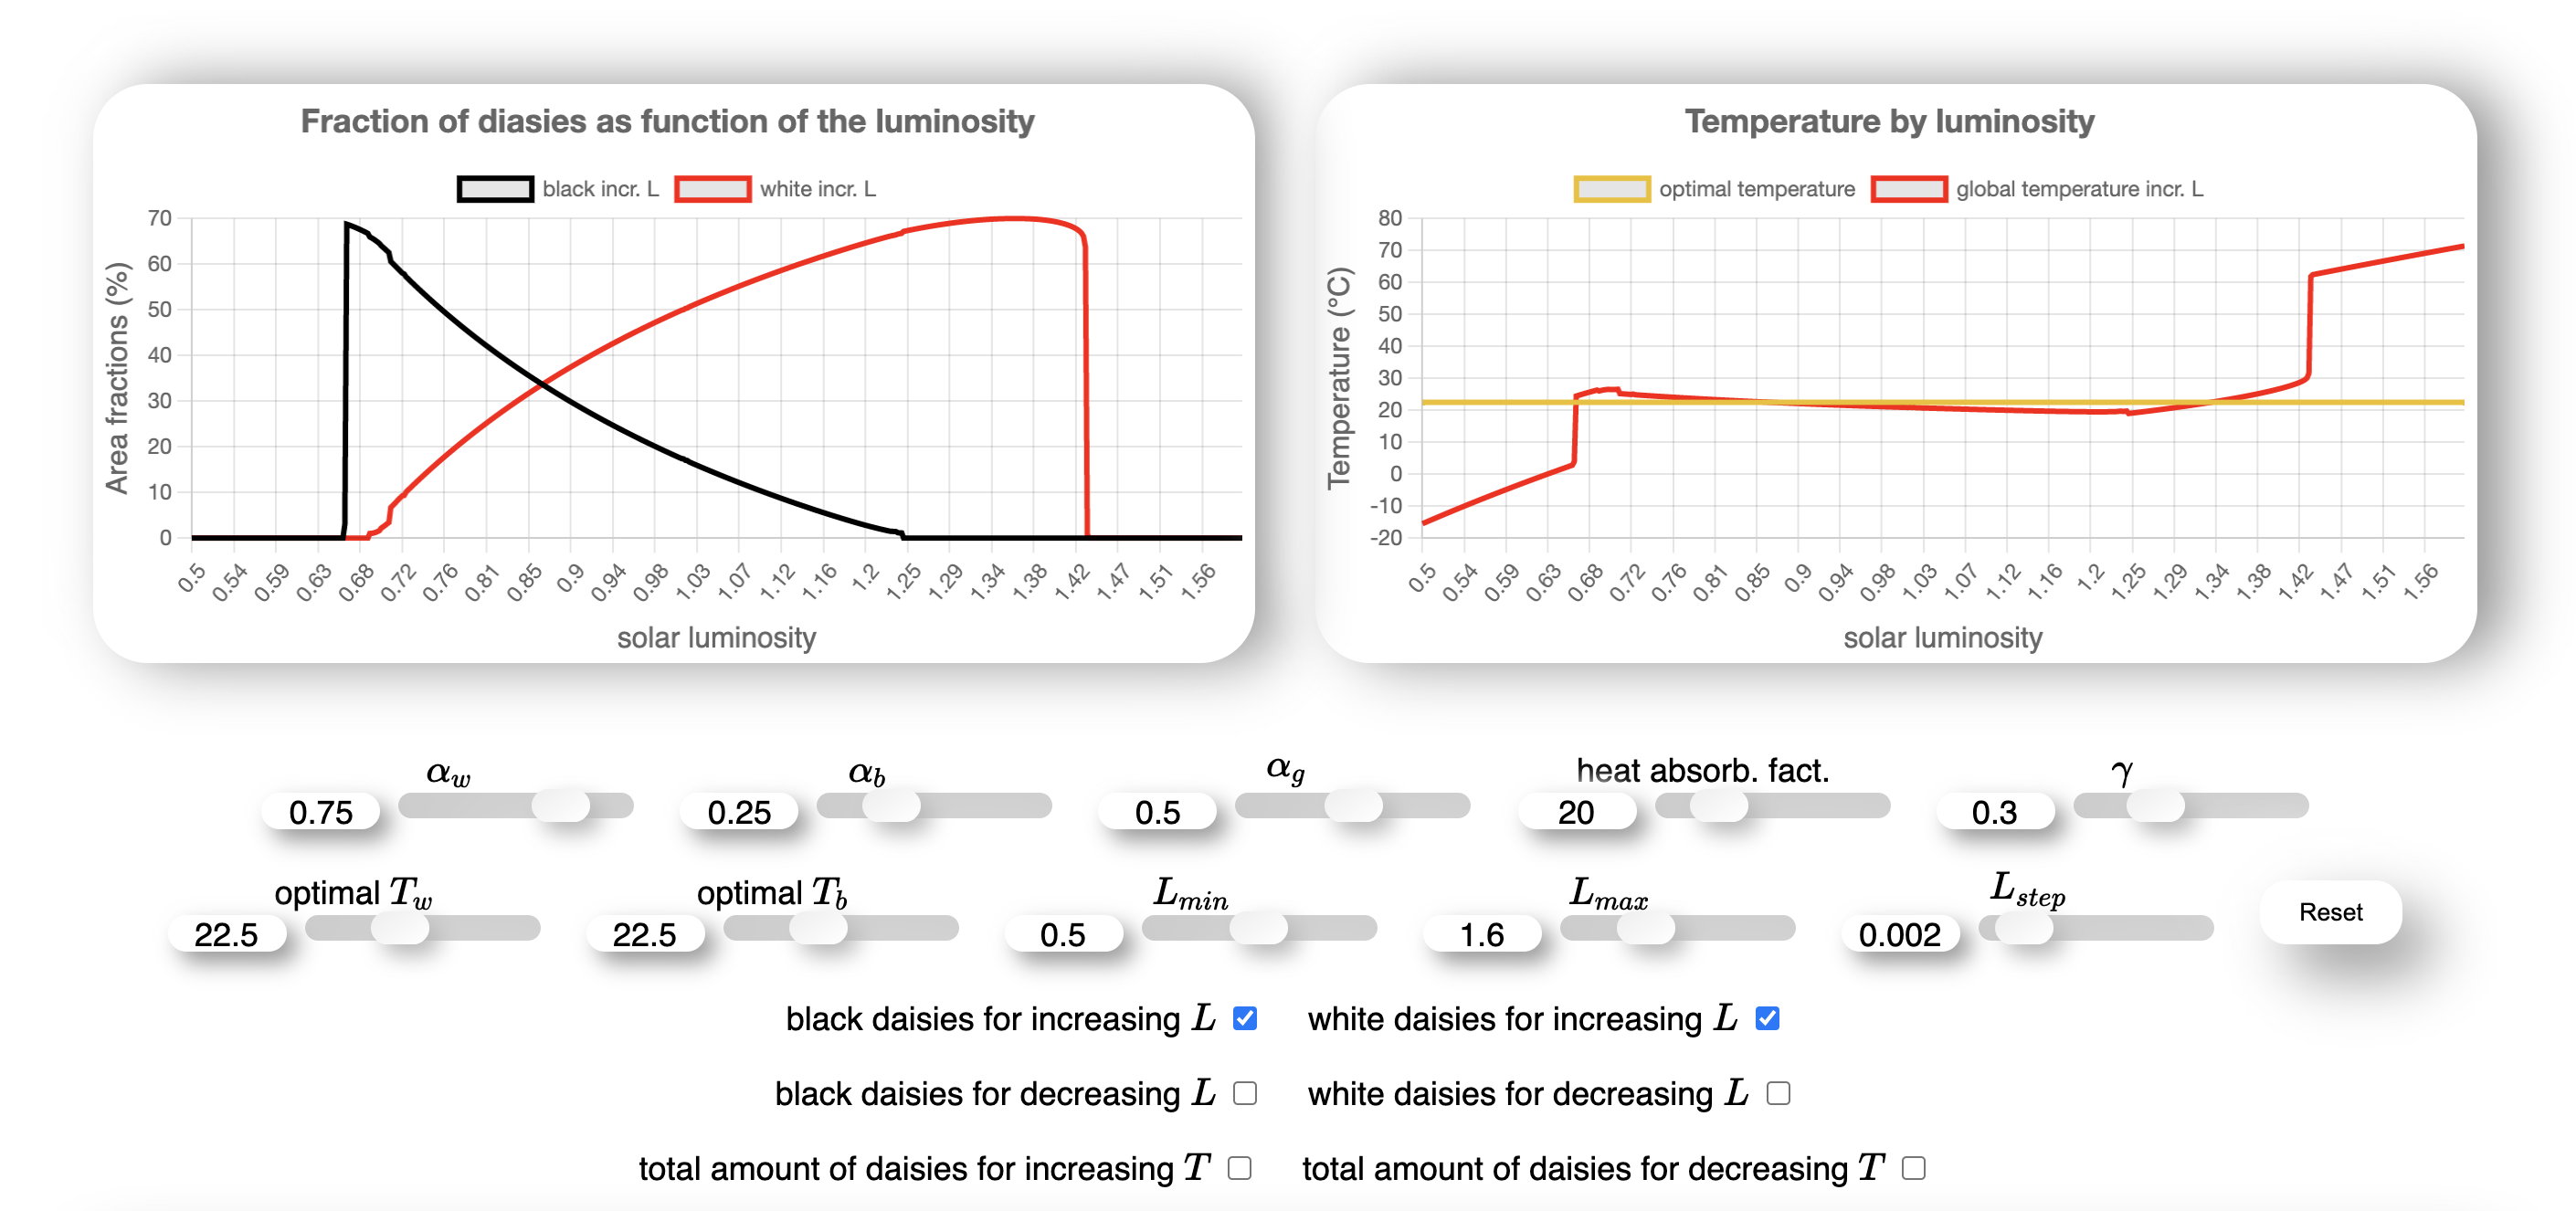
\includegraphics[width=1\linewidth]{daisyworld.png}
\captionof{figure}{\color{Green} Ineractive section of the Daisyworld website with sliders to adjust the parameters and direct visualization of the results. left: distribution of the daisies, right: temperature of the planet at different levels of solar luminosity.}
\end{center}\vspace{1cm}

On this page you also have the possibility to add different graphs and to adjust parameters like the albedo or the death rate.

\subsection{Random system and brownian motion}
For the topics random systems and brownian motion, there are two websites where various interactive graphics can be used to better understand, for example, linear stochastic equations, 2D diffusion and many more.

\begin{center}\vspace{1cm}
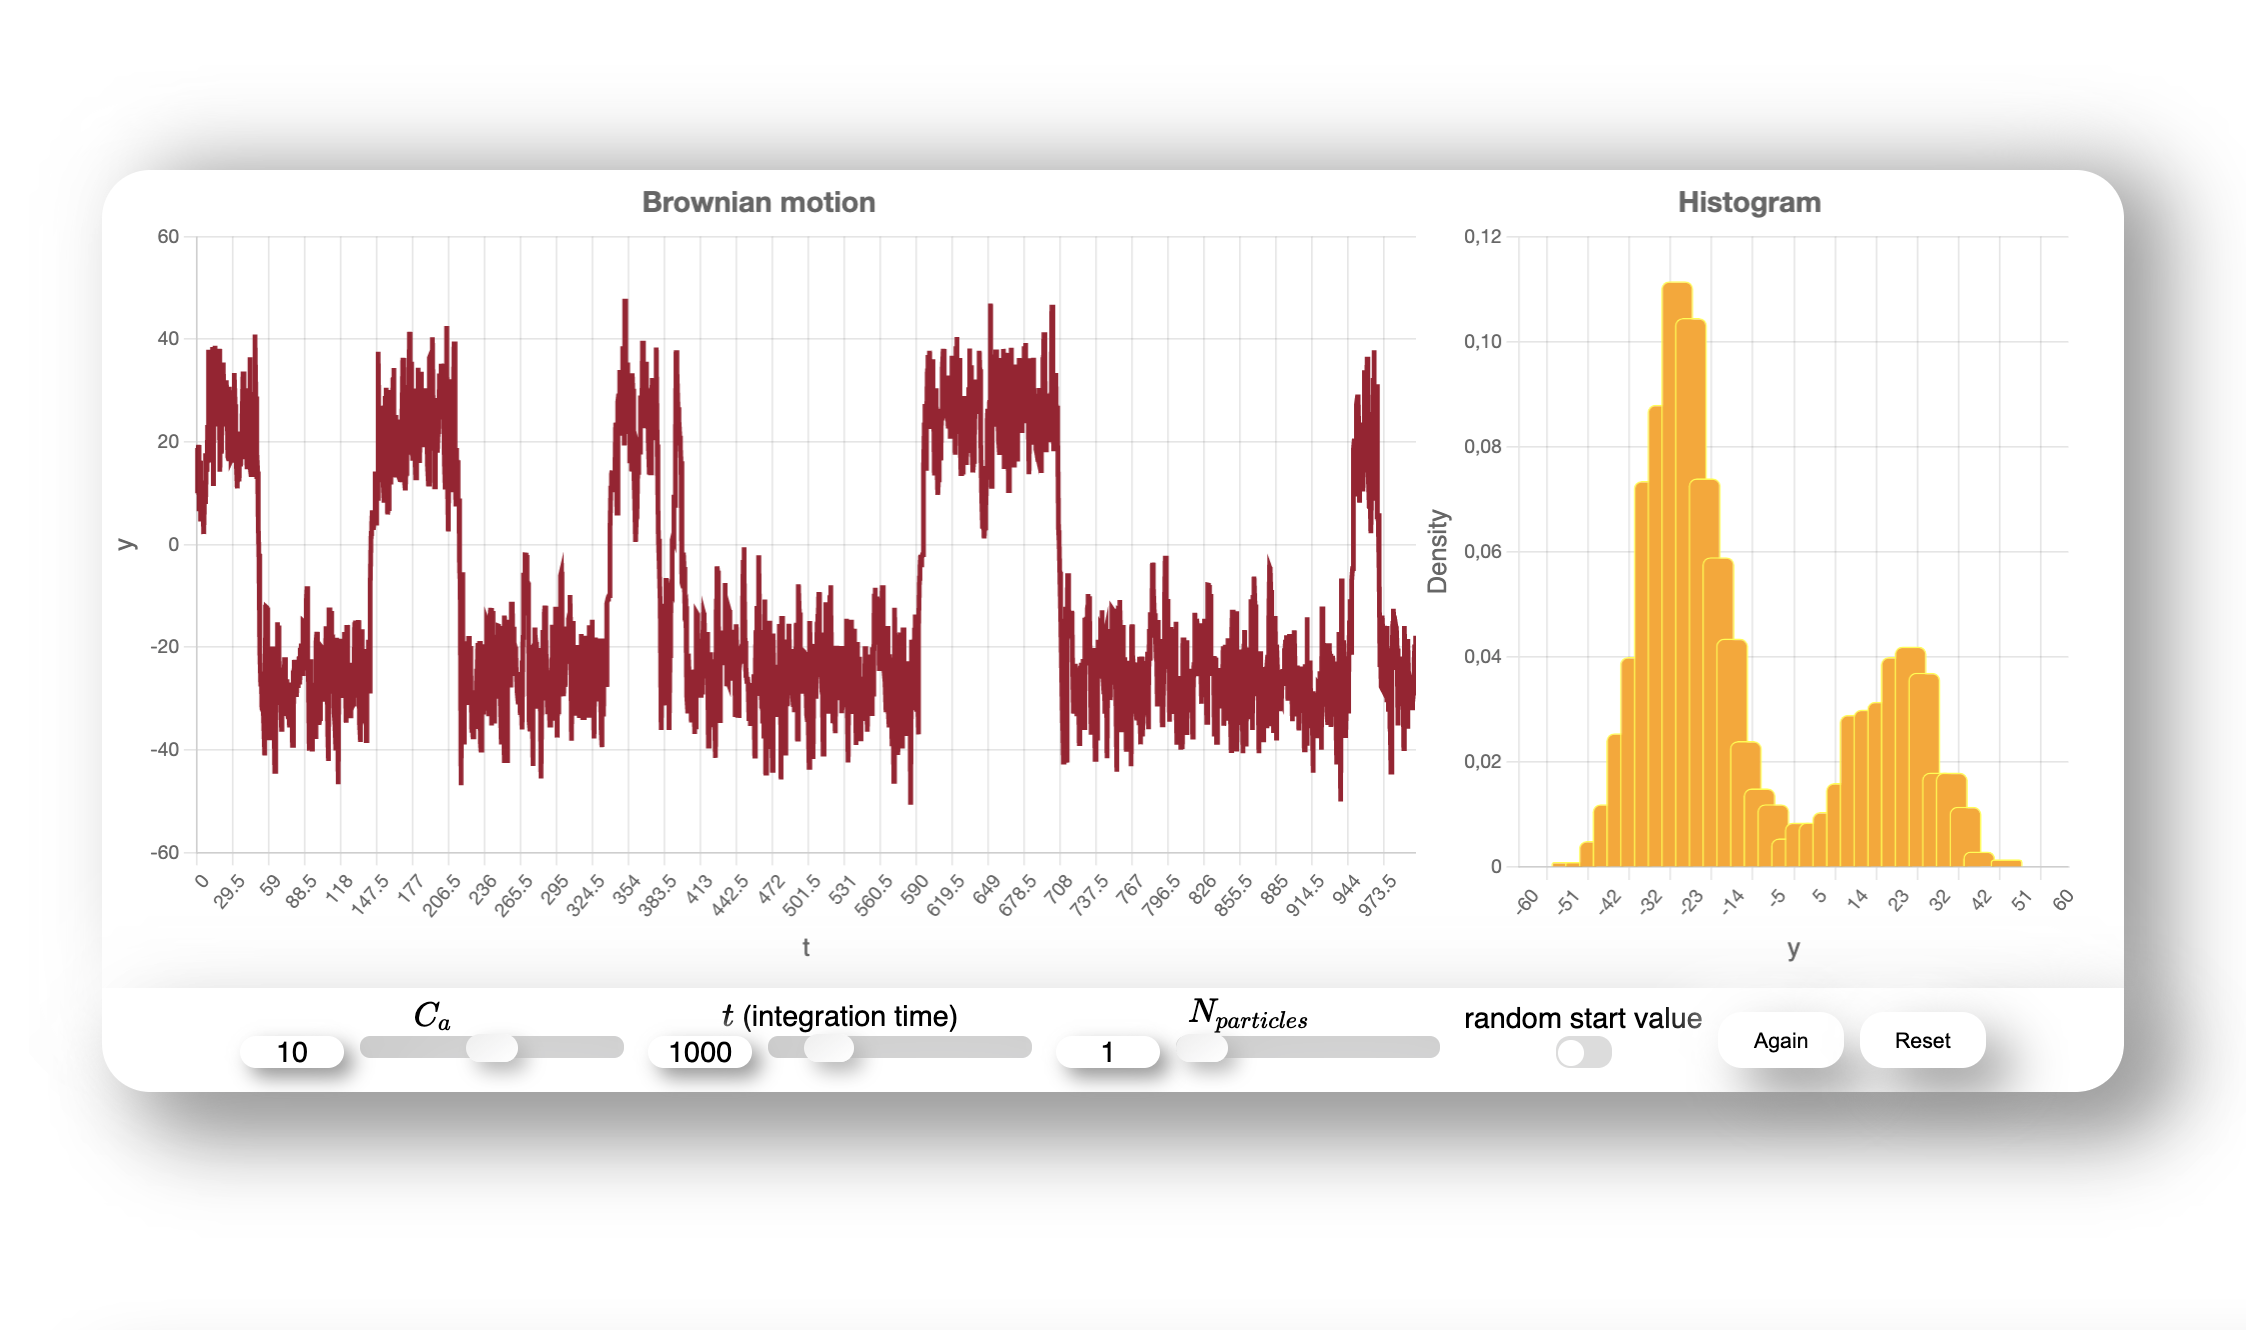
\includegraphics[width=0.8\linewidth]{bm2.png}
\captionof{figure}{\color{Green} Interactive plot of the brownian motion with histogram}
\end{center}\vspace{1cm}

Different configurations can be entered and visualized. The distribution of \(n\) different particles and timesteps can also be visualized and adjusted on additional diagrams.

\begin{center}\vspace{1cm}
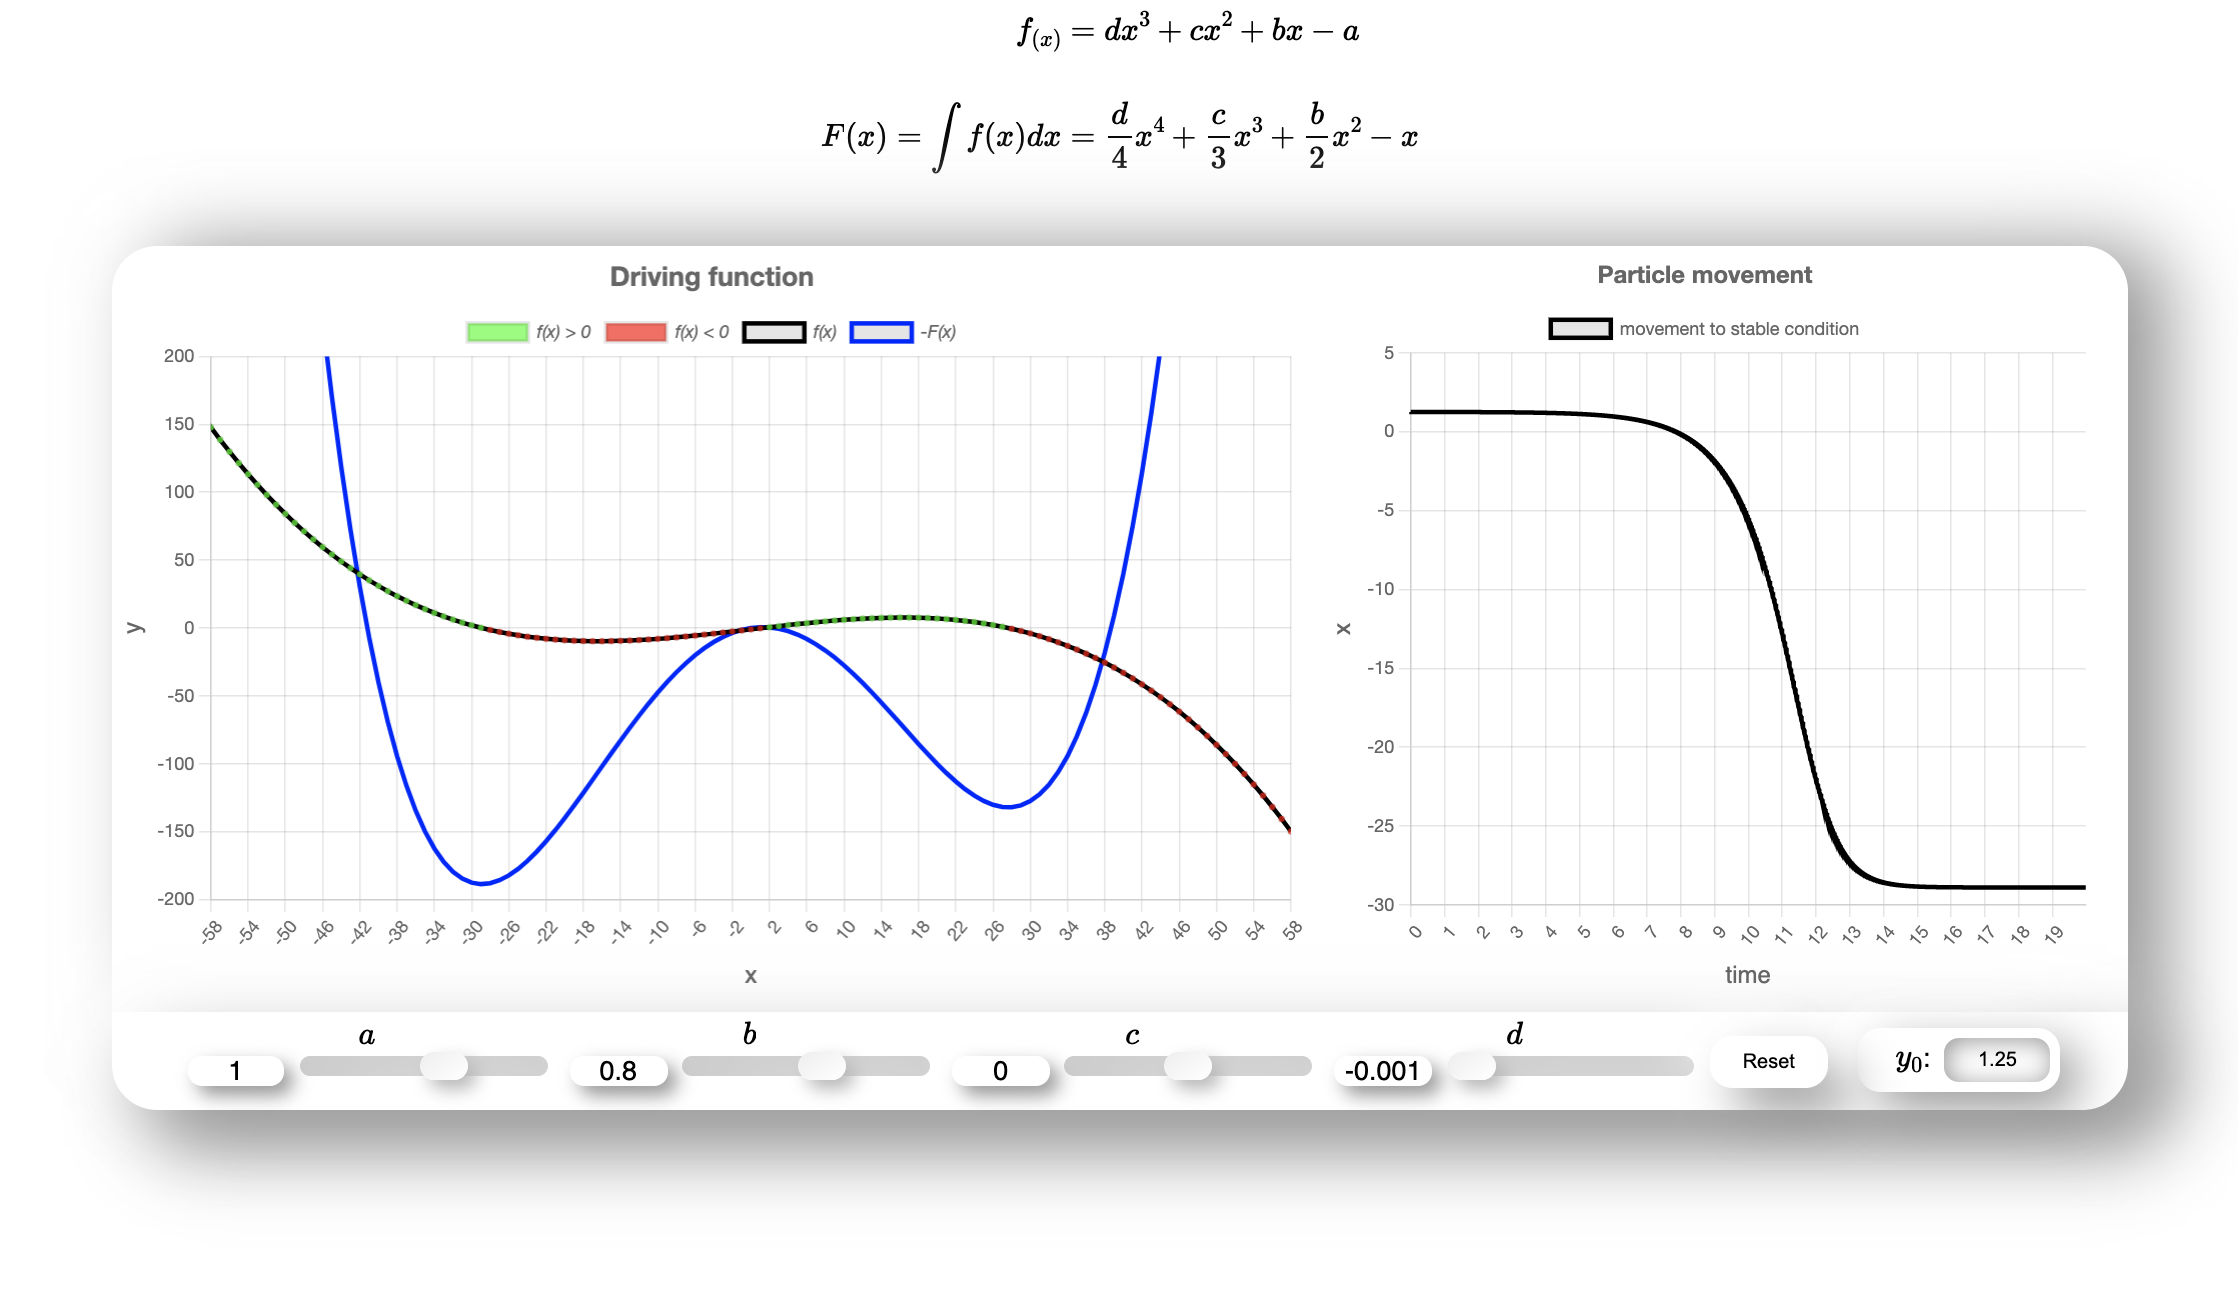
\includegraphics[width=.9\linewidth]{bmdf1.png}
\captionof{figure}{\color{Green} Interactive plot of the driving function of the brownian motion}
\end{center}\vspace{1cm}
On the individual pages you will also find useful notes, definitions, and links to Python source codes and referenced papers.

%----------------------------------------------------------------------------------------
%	CONCLUSIONS
%----------------------------------------------------------------------------------------

\color{SaddleBrown} % SaddleBrown color for the conclusions to make them stand out

\section*{Conclusions}
I have been able to work in different areas of development and analysis and I am looking forward to further challenges. Especially the web development has pleased me very much, hopefully there will be more projects. I would be very happy about questions, comments or project ideas. 
\color{Black} % Set the color back to DarkSlateGray for the rest of the content


 %----------------------------------------------------------------------------------------
%	REFERENCES
%----------------------------------------------------------------------------------------

%\nocite{*} % Print all references regardless of whether they were cited in the poster or not

\bibliographystyle{plain} % Plain referencing style
\bibliography{references}

%----------------------------------------------------------------------------------------

\end{multicols}
\end{document}